%--------------------------------------
% Primary-vertex reconstruction
%--------------------------------------
\section{Primary vertex and diffuse offset energy density}
\subsection{Primary vertex}
\label{s:secPV}
    To reconstruct a primary vertex (PV) following three steps are performed~\cite{Chatrchyan:2014fea}:
    \begin{itemize}[leftmargin=*]
        \item {\bf{ Track selection}}: Primary vertices are associated with a large number of tracks
            emerging from the same point. Tracks satisfying following criteria are used to reconstruct the collision point (vertex). 
           \begin{itemize}[leftmargin=*]
               \item distance of closest approach from the center of beamspot $< 2.4$ \unit{cm},
               \item number of the associated pixel hits $\geq 2$, and
               \item number of the associated pixel+strips hits $\geq 5$.
           \end{itemize}
      \item {\bf{ Track clustering}}: After track selection, the level of association of tracks 
	from a vertex is quantified. This procedure is called track clustering where tracks are 
	clustered according to their $z$-position from the center of beamspot. The Deterministic 
	Annealing algorithm~\cite{an-11-014, 726788} is used for such clustering. After clustering, 
	the candidate vertices are found along with the tracks associated with them.
      \item {\bf{ Vertex-position fitting}}: The $z$-position of candidate vertices with at least two 
	tracks are fitted using the {\em adaptive vertex fitter}~\cite{Fruhwirth:1027031}. The fit 
	returns $x$, $y$, $z$-position, and covariance matrix of the PV along with other parameters 
	such as the number of degrees of freedom ($n_{\rm {dof}}$) and a weight associated with each 
	track. We require $n_{\rm {dof}} > 4$.
   \end{itemize}

The simulated samples listed in Table~\ref{tab:mcSample} were generated before the actual data 
taking in 2016. While simulating these samples, the pileup distribution as initially seen in the 
data was used. During the actual data taking, however, the pileup distributions were changed.
To have a similar pileup distribution as in data, the simulated events are re-weighted.
After applying the pileup weights, as discussed in Section~\ref{s:pileup_reweighting}, the distribution of number of primary vertices per event 
($\rm{N}^{\text{vertex}}$) is shown in Figures~\ref{subfig:nvtx_muKinFit} and \ref{subfig:nvtx_eleKinFit} 
for the \mujets and \ejets channel, respectively.

\subsection{Diffuse offset energy density}
From Figures~\ref{subfig:nvtx_muKinFit} and \ref{subfig:nvtx_eleKinFit}, it can be seen that there 
is a poor agreement between data and simulation even after applying the pileup reweighting.
A similar trend is seen in many analyses at 13 \TeV~\cite{CMS-AN-17-003, CMS-AN-17-116}. There 
is another variable similar to $\rm{N}^{\text{vertex}}$ called diffuse offset energy density
($\rho$)~\cite{Cacciari:2005hq, Cacciari:2011ma}. For $n$ number of jets in an event, $\rho$ is 
given by~\cite{Cacciari:2007fd}
\begin{equation}
    \rho = {\text{median}}\left(\frac{p_{T, n}}{A_n}\right)
    \label{eq:rho}
\end{equation}
where $p_{T,n}$ and $A_n$ are the transverse momentum and area of $n^{\text{th}}$ jet.
The $\rho$ distribution is shown in Figures~\ref{subfig:rhoAll_muKinFit} and \ref{subfig:rhoAll_eleKinFit}. It can be seen that $\rho$ has a better agreement between data and simulation as compared to the 
$\rm{N}^{\text{vertex}}$ distribution. The $\rho$ is used in the calculation of isolation variable for 
muon and electron as shown in Equation (\ref{eq:ele_iso}). The jet energy corrections are also 
derived using $\rho$ as discussed in Section~\ref{ss:jet_id}.

\begin{figure}
    \centering  
    \subfigure[\label{subfig:nvtx_muKinFit}]
    {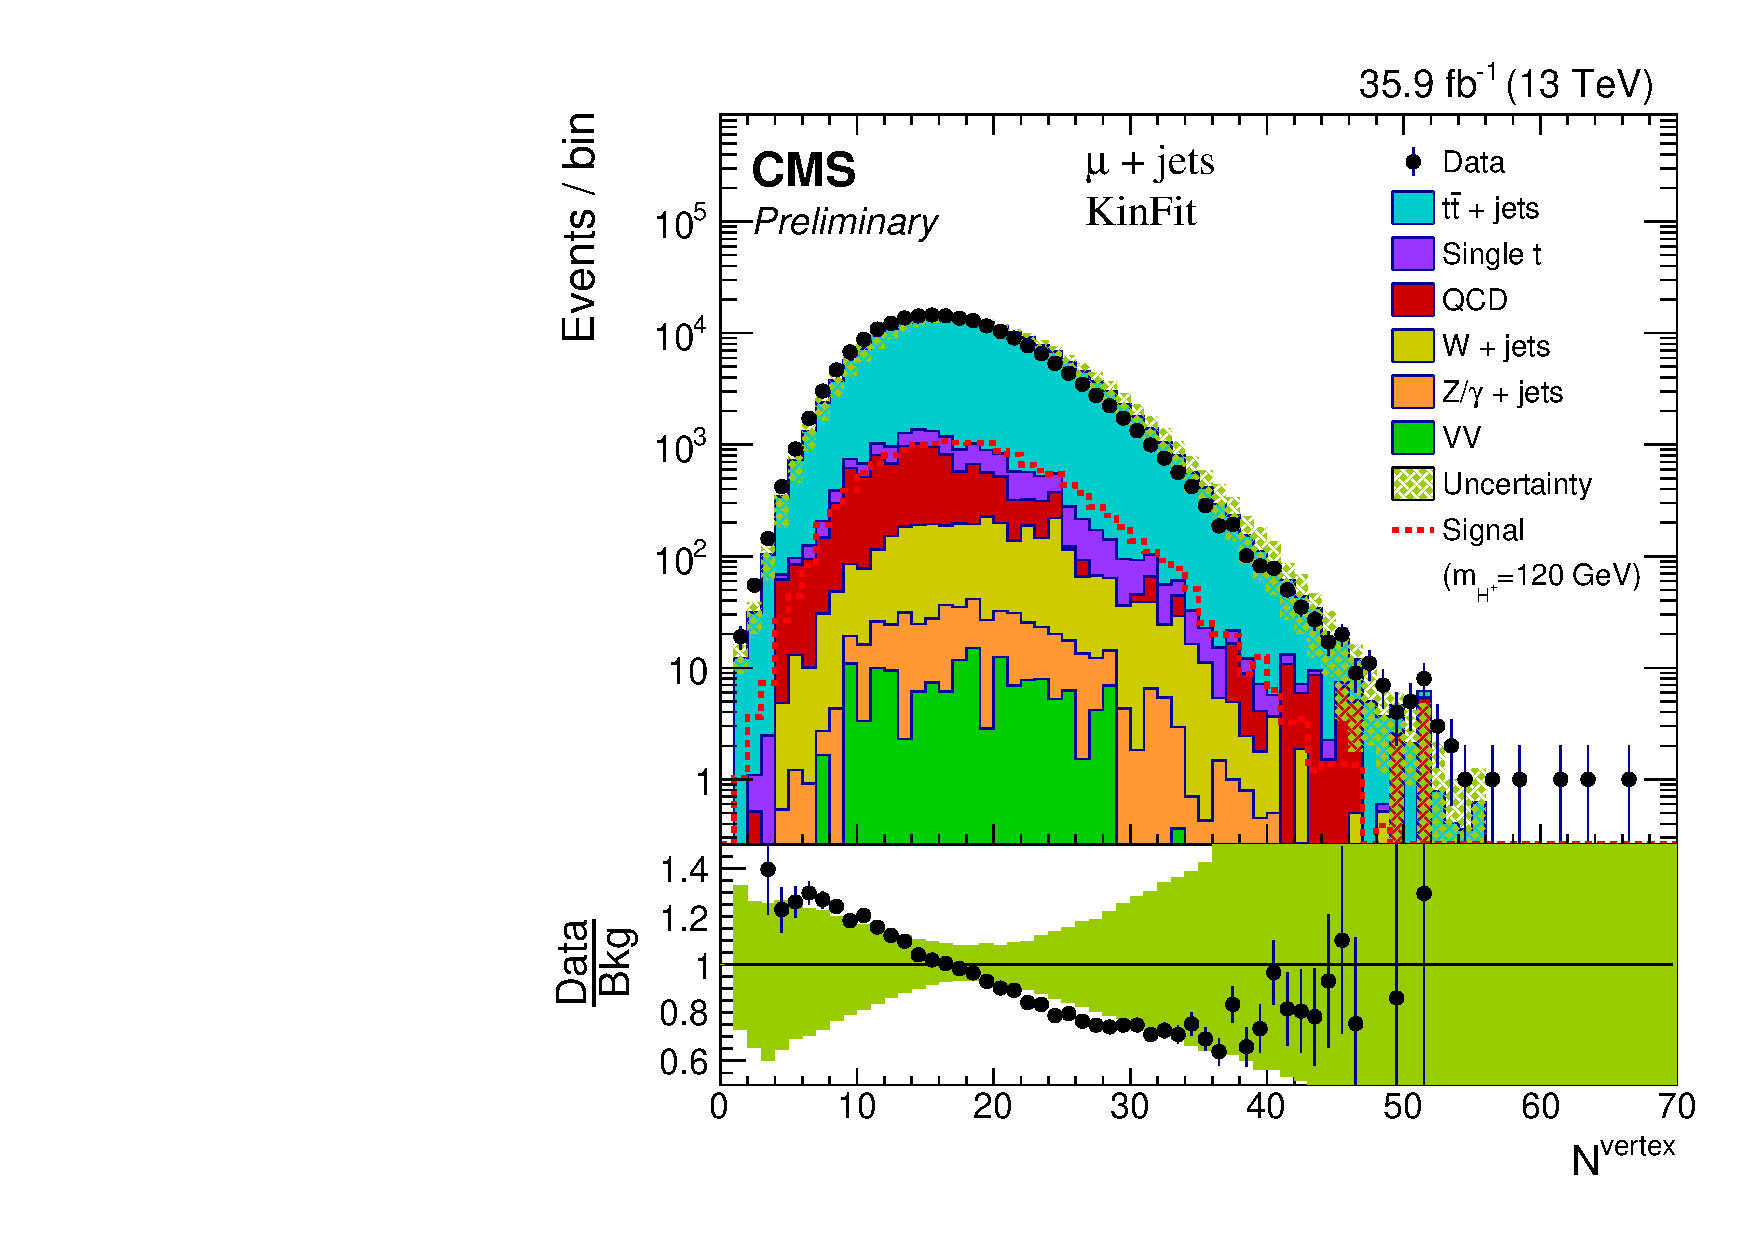
\includegraphics[width=0.49\linewidth]{Image/Muon/KinFit/nvtx_muKinFit.pdf}}
    \subfigure[\label{subfig:nvtx_eleKinFit} ]
    {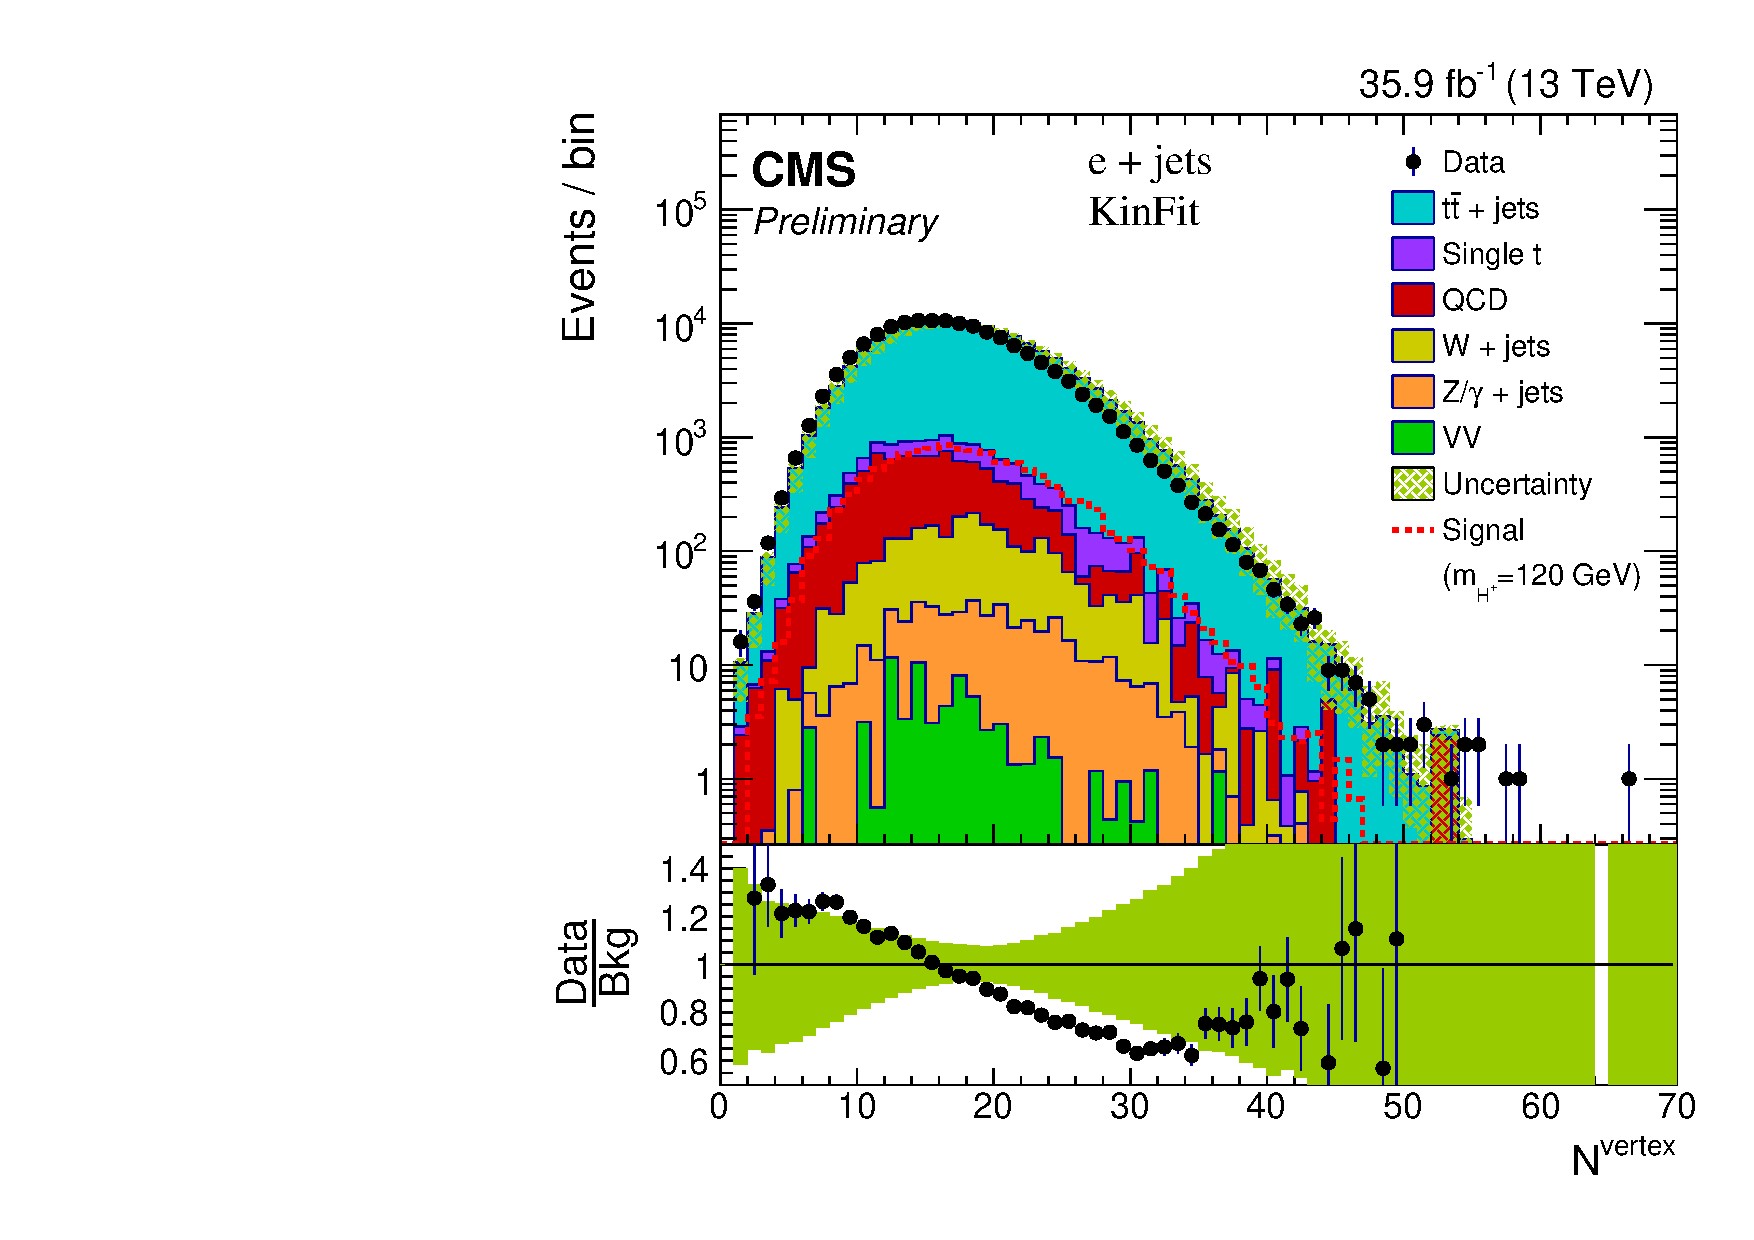
\includegraphics[width=0.49\linewidth]{Image/Electron/KinFit/nvtx_eleKinFit.pdf}}
    \vfil
    \subfigure[\label{subfig:rhoAll_muKinFit}]
    {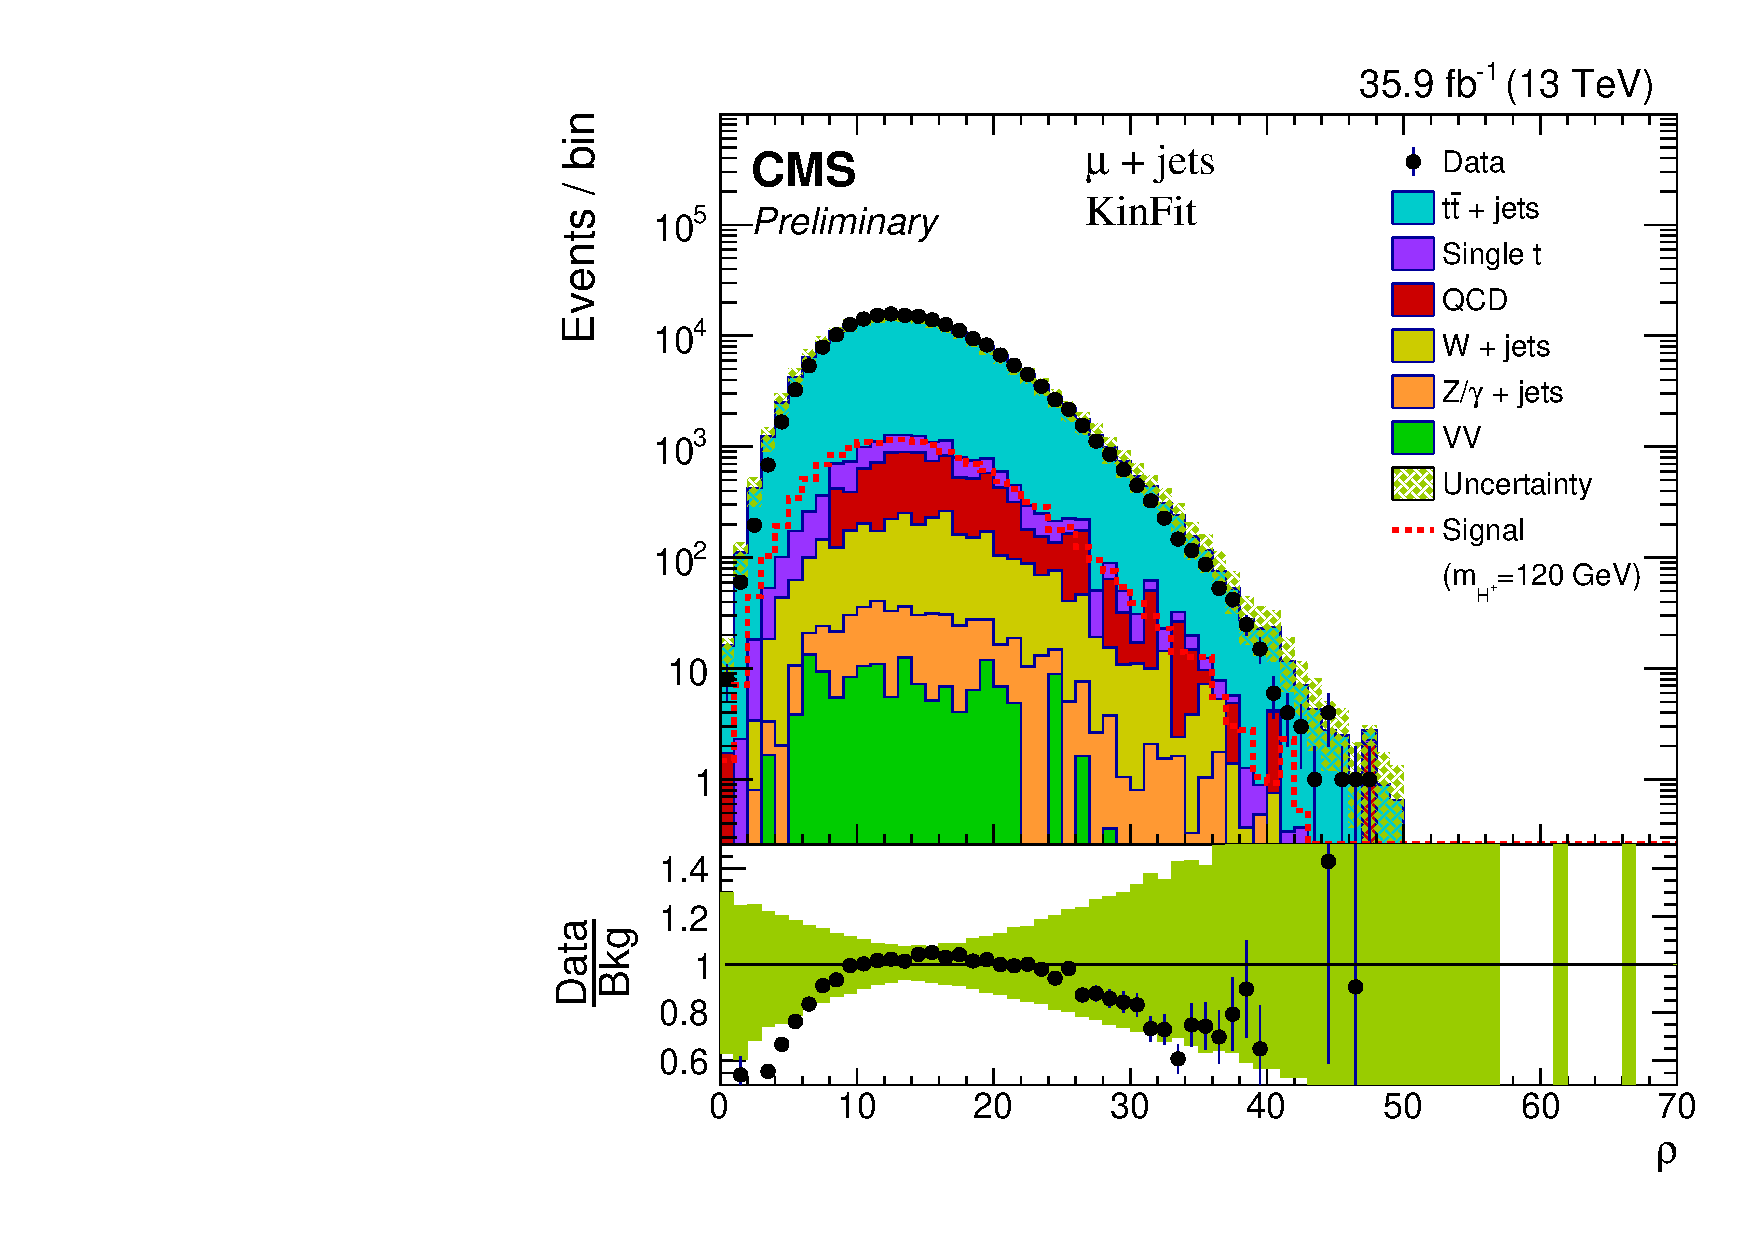
\includegraphics[width=0.49\linewidth]{Image/Muon/KinFit/rhoAll_muKinFit.pdf}}
    \subfigure[\label{subfig:rhoAll_eleKinFit}]
    {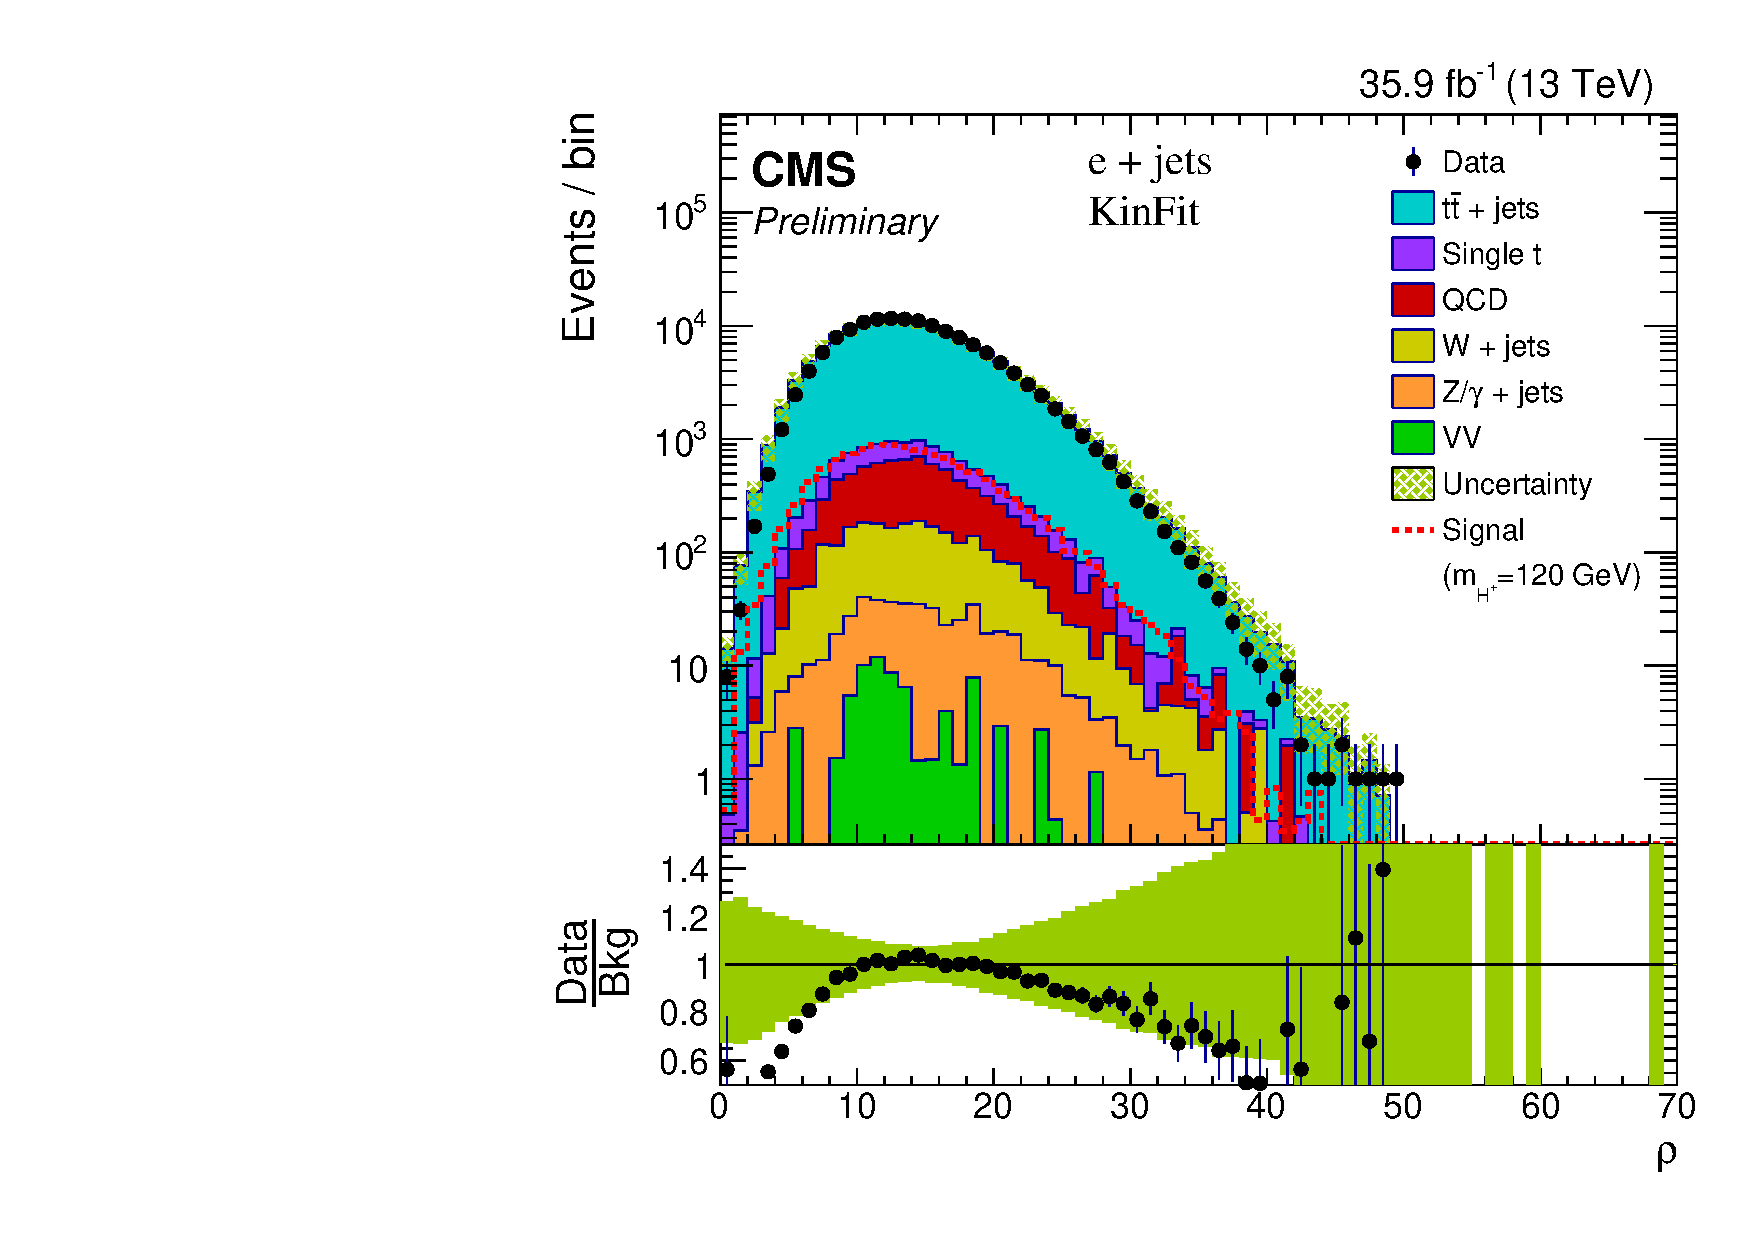
\includegraphics[width=0.49\linewidth]{Image/Electron/KinFit/rhoAll_eleKinFit.pdf}}
    \caption{Distribution of number of primary vertices and diffuse offset energy density 
	for \mujets and \ejets channels. The agreement between data and simulation is better 
	for $\rho$ as compared to $\rm{N}^{\text{vertex}}$ distribution. However, for lower values 
	of $\rho$, there is a significant mismatch between data and simulation. Similar trend is 
	seen in other analysis as well~\cite{CMS-AN-17-003, CMS-AN-17-116}.}
    \label{fig:nvtxRho}
\end{figure}

%--------------------------------------
% Muon Reconstruction
%--------------------------------------
\section{Muon}
\label{s:muReco}
\subsection{Reconstruction}
Muons are often referred to as minimum ionising particles. Their energy loss is much smaller than 
electrons due to its larger mass. Muon in CMS detector with sufficiently higher \pt can traverse 
through most of the sub-detectors such as tracker, calorimeter, and the muon chambers. Most of the 
high $\pt$ muons go out of the CMS detector. Due to the presence of a magnetic field, trajectories 
of muon are bent in the CMS detector. The number of hits in the tracker, energy deposit in the 
calorimeter and the hits in the muon chambers (DT, CSC, and RPC) are used in the Kalman filtering (KF) 
technique~\cite{FRUHWIRTH1987444} to reconstruct muon candidates. There are several categories of 
muons~\cite{Chatrchyan:2012xi} described below:
\begin{itemize}[leftmargin=*]
   \item {\bf{ Standalone muons}}: These are reconstructed from the muon chambers only. Here, the
       KF technique uses the hits from DT, CSC, and RPC to reconstruct standalone muons.
   \item {\bf{ Global muons}}: The trajectory of a standalone muon is extrapolated up to the tracker. 
       The best pair consisting of the standalone muon and tracker track is selected using the
       KF technique. Finally, these two tracks are combined to reconstruct global muon.
       As the global muons are reconstructed starting from the outer part (muon chambers) of the CMS 
	detector back to the inner part (strip tracker), this approach of reconstruction is called 
       {\em outside-in}.
   \item {\bf{ Tracker muons}}: There is an {\em inside-out} approach to reconstruct muons, which 
       starts from the tracks reconstructed in the strip tracker to the energy deposits in the calorimeters
       up to the hits in the muon chamber. Muons reconstructed with this approach are called tracker muons.
   \item {\bf{ RPC muons}}: These muons are also reconstructed using the {\em inside-out} approach 
       where only RPC hits of the muon chamber are used~\cite{Goh:2014tra}. 
   \item {\bf{ Calorimeter muons}}: Some of the reconstructed muon tracks consist of energy deposits
       from the calorimeters. Such muons are called calorimeter muons.
\end{itemize}

\subsection{Identification and selection}
In the event topology of our interest, there only one lepton (electron or muon) as shown in Figure~\ref{fig:feyn_diag_sig}. These are the 'prompt' lepton coming
directly from the electroweak decay of \PW bosons. However, there could be 'extra'
leptons that come from other sources such as misidentification of light flavored
jets or charged pion decay in case of muons. Medium identification (ID) criteria, as 
listed Table~\ref{tab:muonSel}, are applied to select prompt muons. 
The efficiency of medium muon ID as a function of
\pt and $\eta$ is shown in Figure~\ref{fig:muonIsoIDEff} from data and simulation.
From this figure, it can be seen that the efficiency at lower \pt is relatively
low compared to that from high \pt. However there is a sudden drop in the
efficiency for data from era BCDEF (The data taking periods are divided in different eras. 
For example, the first few months after the data taking starts are assigned era-A and so on. Note that some of the eras may have number of days less than 30) 
in the $\pt > 120$ \GeV region. 
\begin{table}
  \caption{Selection and veto cuts applied on muon.}
 \begin{center}
 \begin{tabular}{ccc}\hline\hline
 Variable & Selection & Veto\\ \hline\hline
 \pt (\GeV) & $> 26 $ & $> 15$\\
 $|\eta|$ & $< 2.4$ & $< 2.4$ \\
 Global or tracker muon & Yes & Global \\
 Normalised $\chi^2$ & $< 3$ & \\
 $\chi^2$ local position & $< 12$ & \\
 Tracker kink & $< 20$ &\\
 Segment compatibility & $ > 0.303 $ & \\
 $|d_\mathrm{xy}(\mathrm{vertex})|$(\unit{cm}) & $< 0.05$ & \\
 $|d_\mathrm{z}(\mathrm{vertex})|$ (\unit{cm}) & $< 0.2$ & \\
 Inner track valid fraction & $> 0.8$ & \\
 $I_{\rm {rel}}^\mu~$ & $< 0.15$ & $< 0.25$\\\hline
 \end{tabular}
 \end{center}
 \label{tab:muonSel}
 \end{table}
\begin{figure}
    \centering
    \subfigure[\label{subfig:muonIDEffPt}]
    {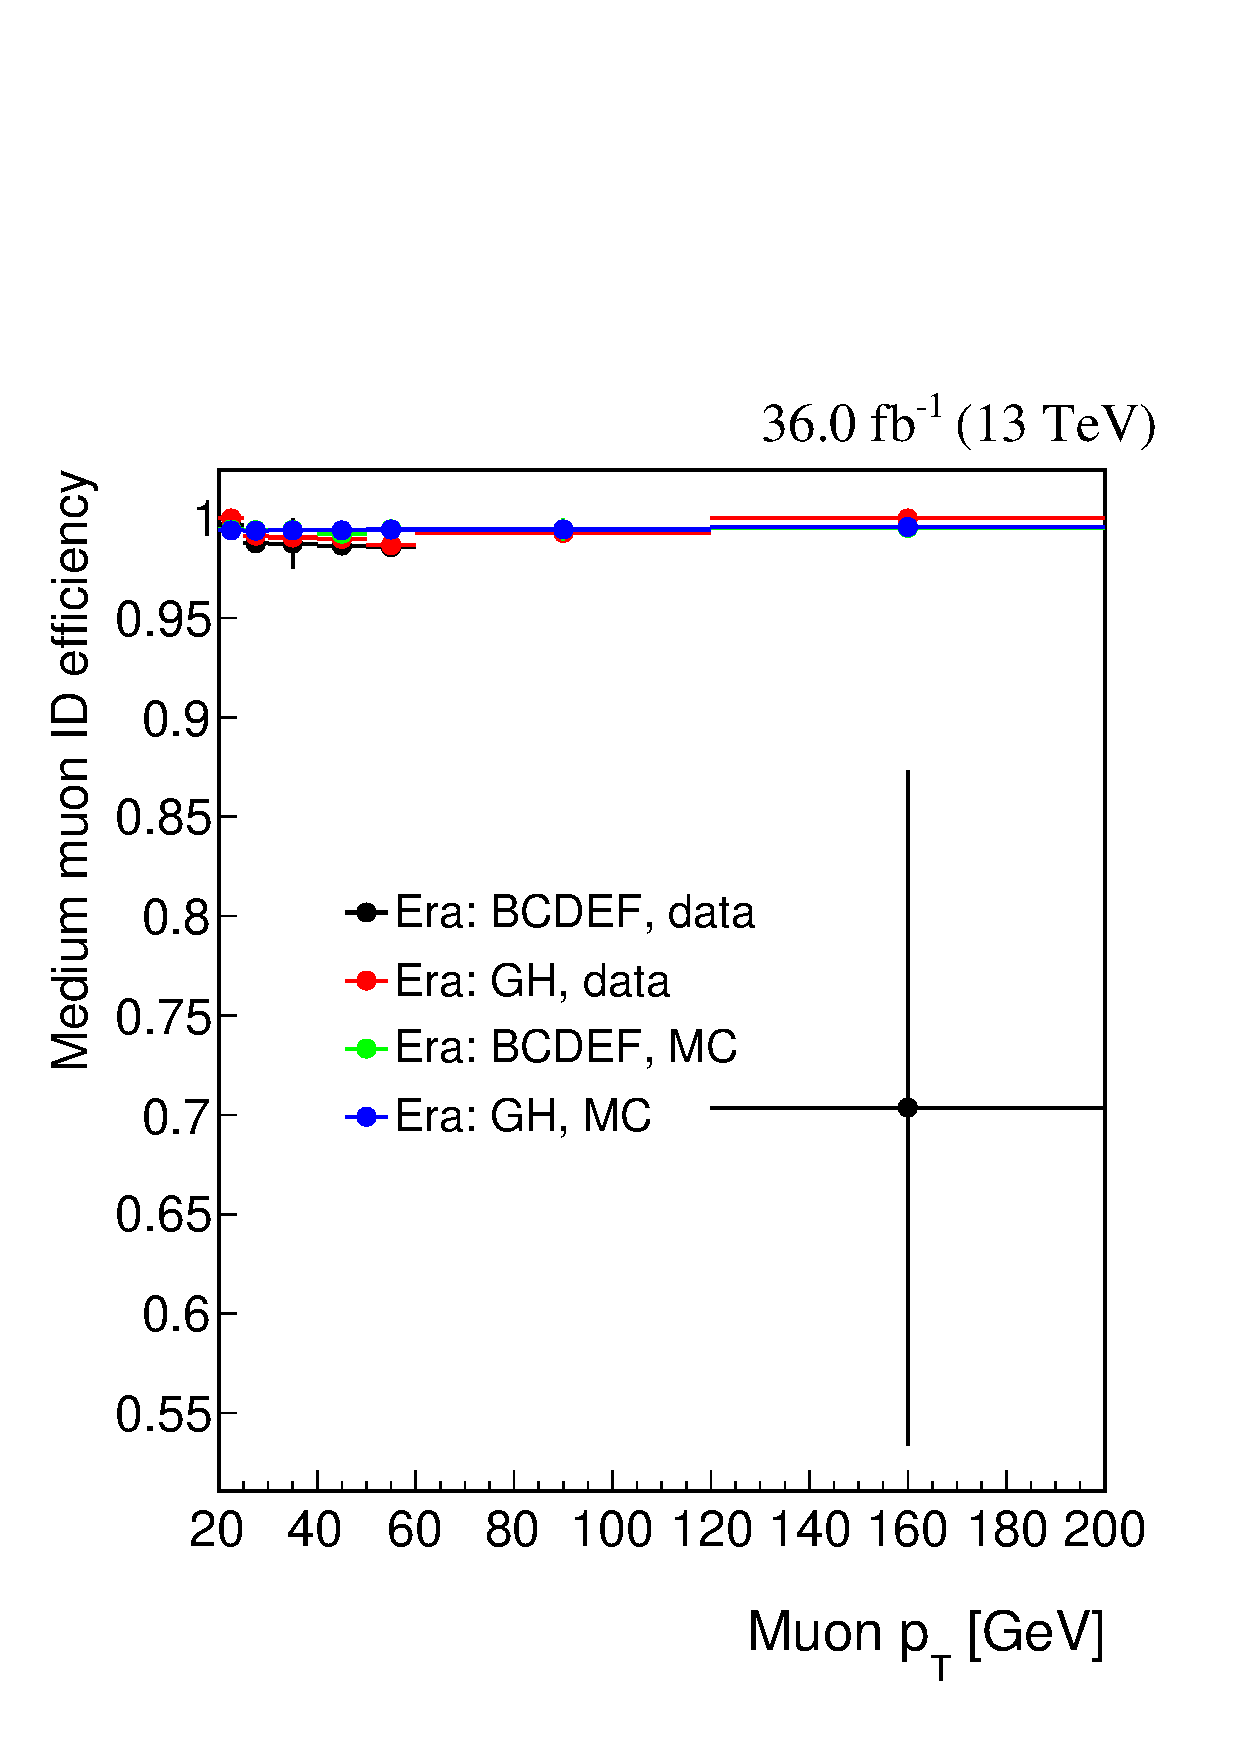
\includegraphics[width=0.45\linewidth]{Image/Muon/muSF_png/muonIDEffPt.pdf}}
    \subfigure[\label{subfig:muonIDEffEta}]
    {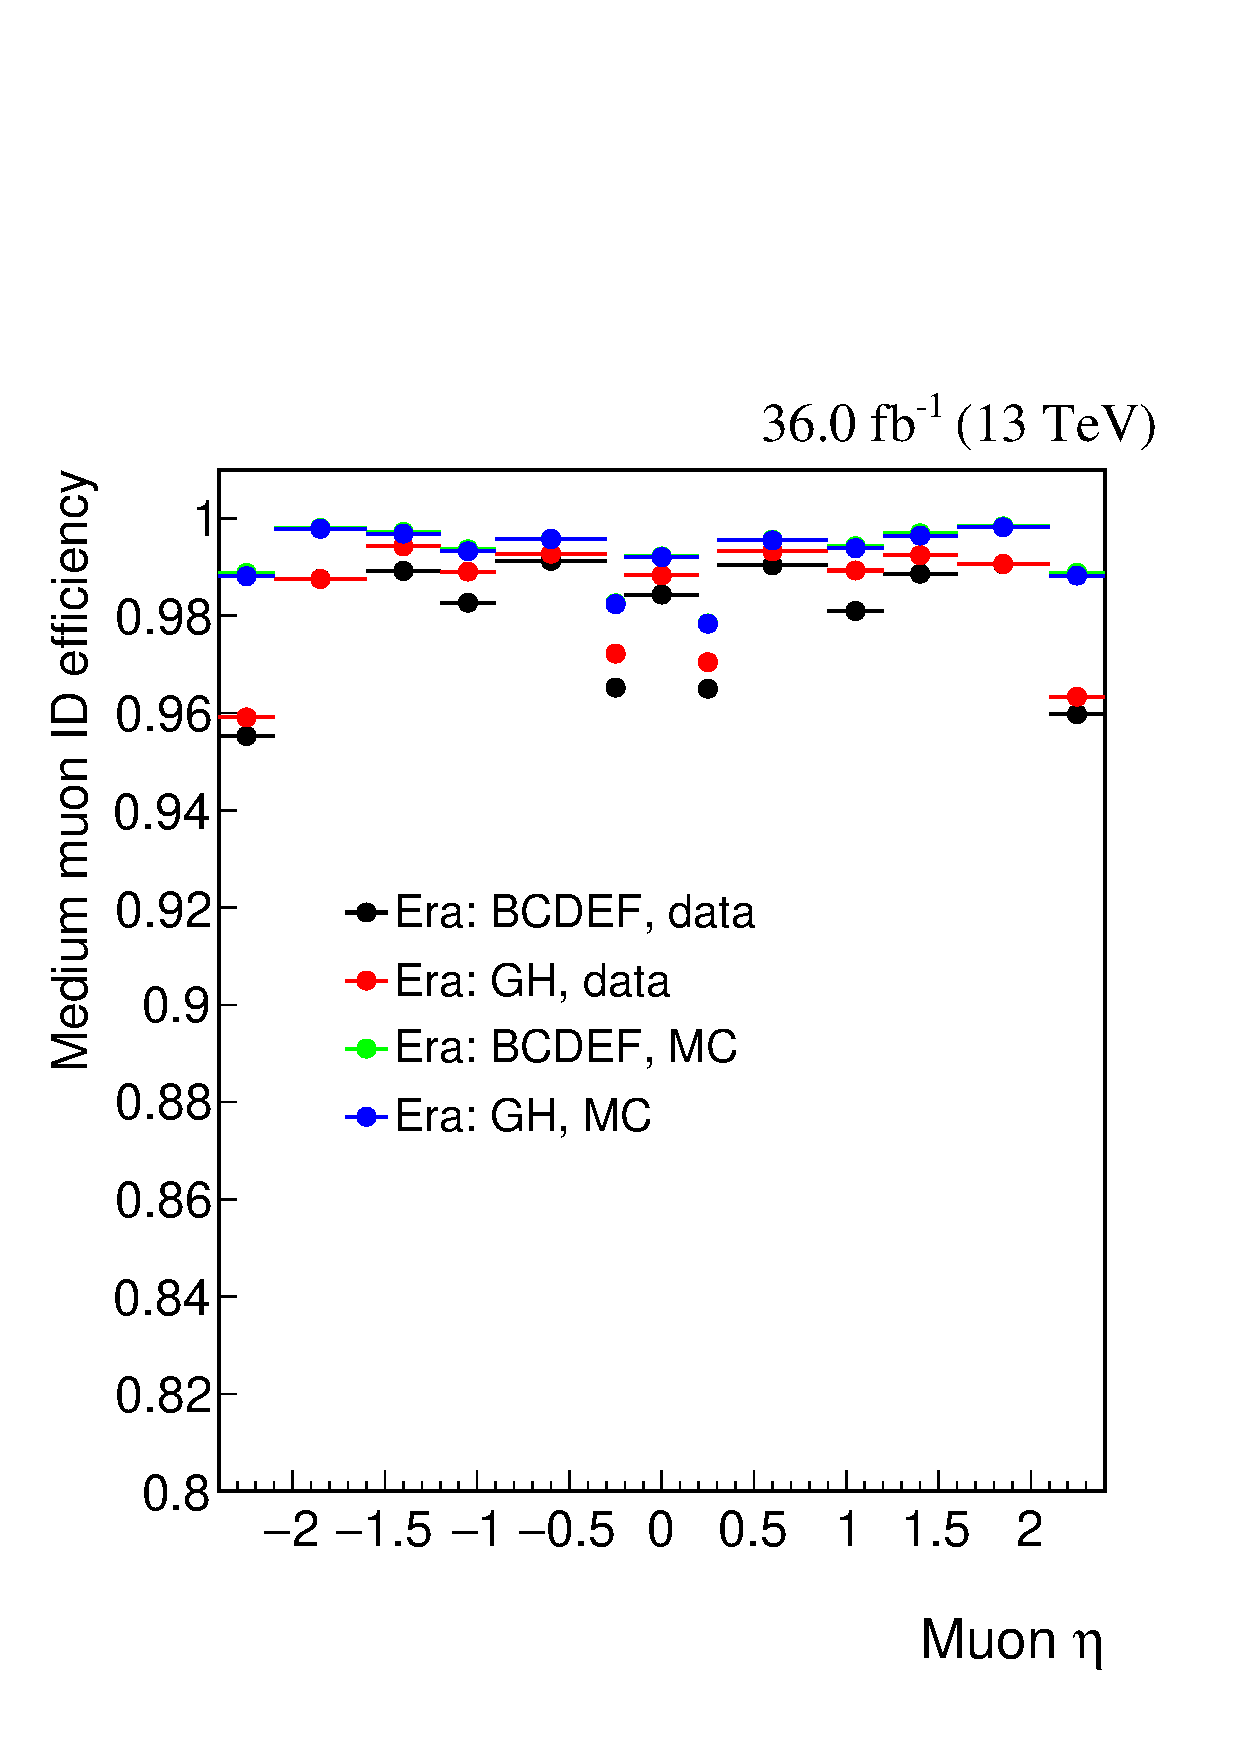
\includegraphics[width=0.45\linewidth]{Image/Muon/muSF_png/muonIDEffEta.pdf}}
    \vfil
    \subfigure[\label{subfig:muonIsoEffPt}]
    {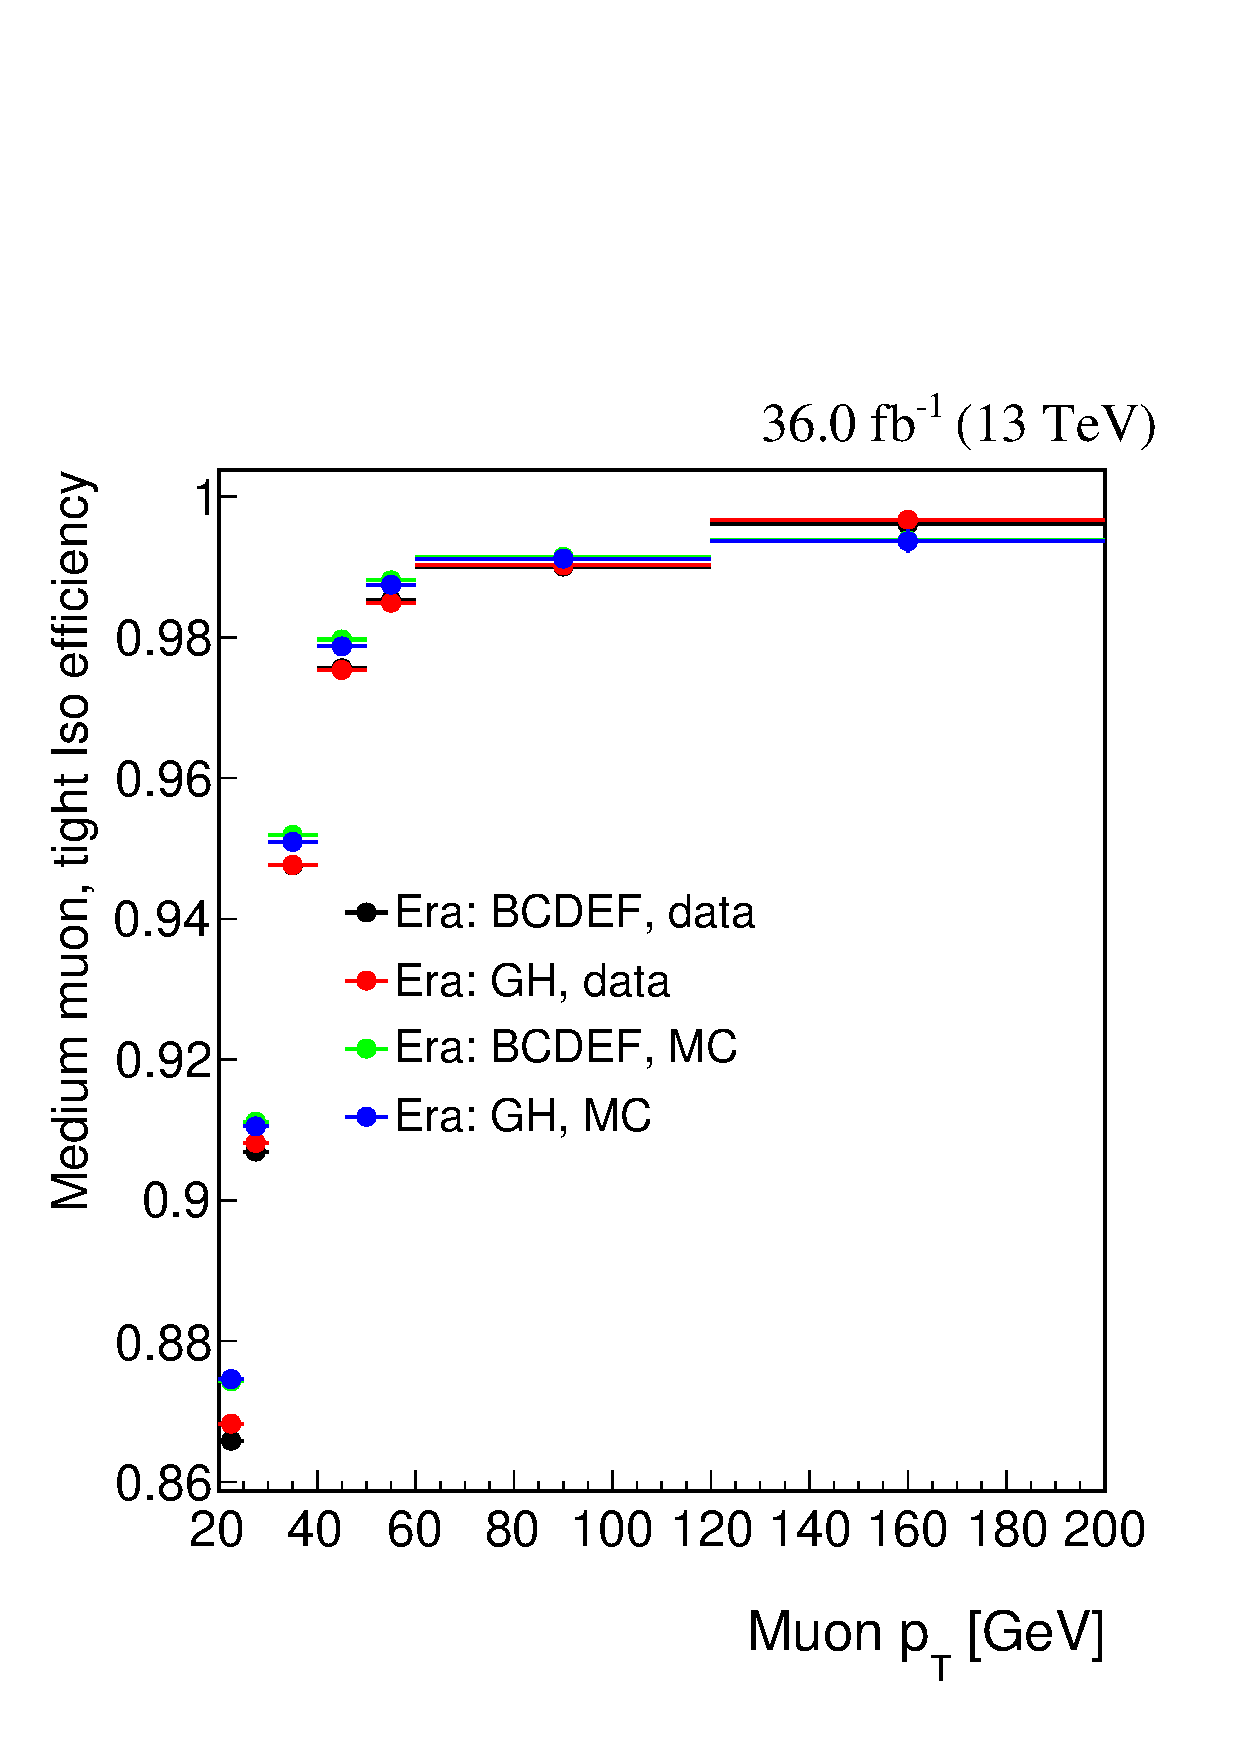
\includegraphics[width=0.45\linewidth]{Image/Muon/muSF_png/muonIsoEffPt.pdf}}
    \subfigure[\label{subfig:muonIsoEffEta}]
    {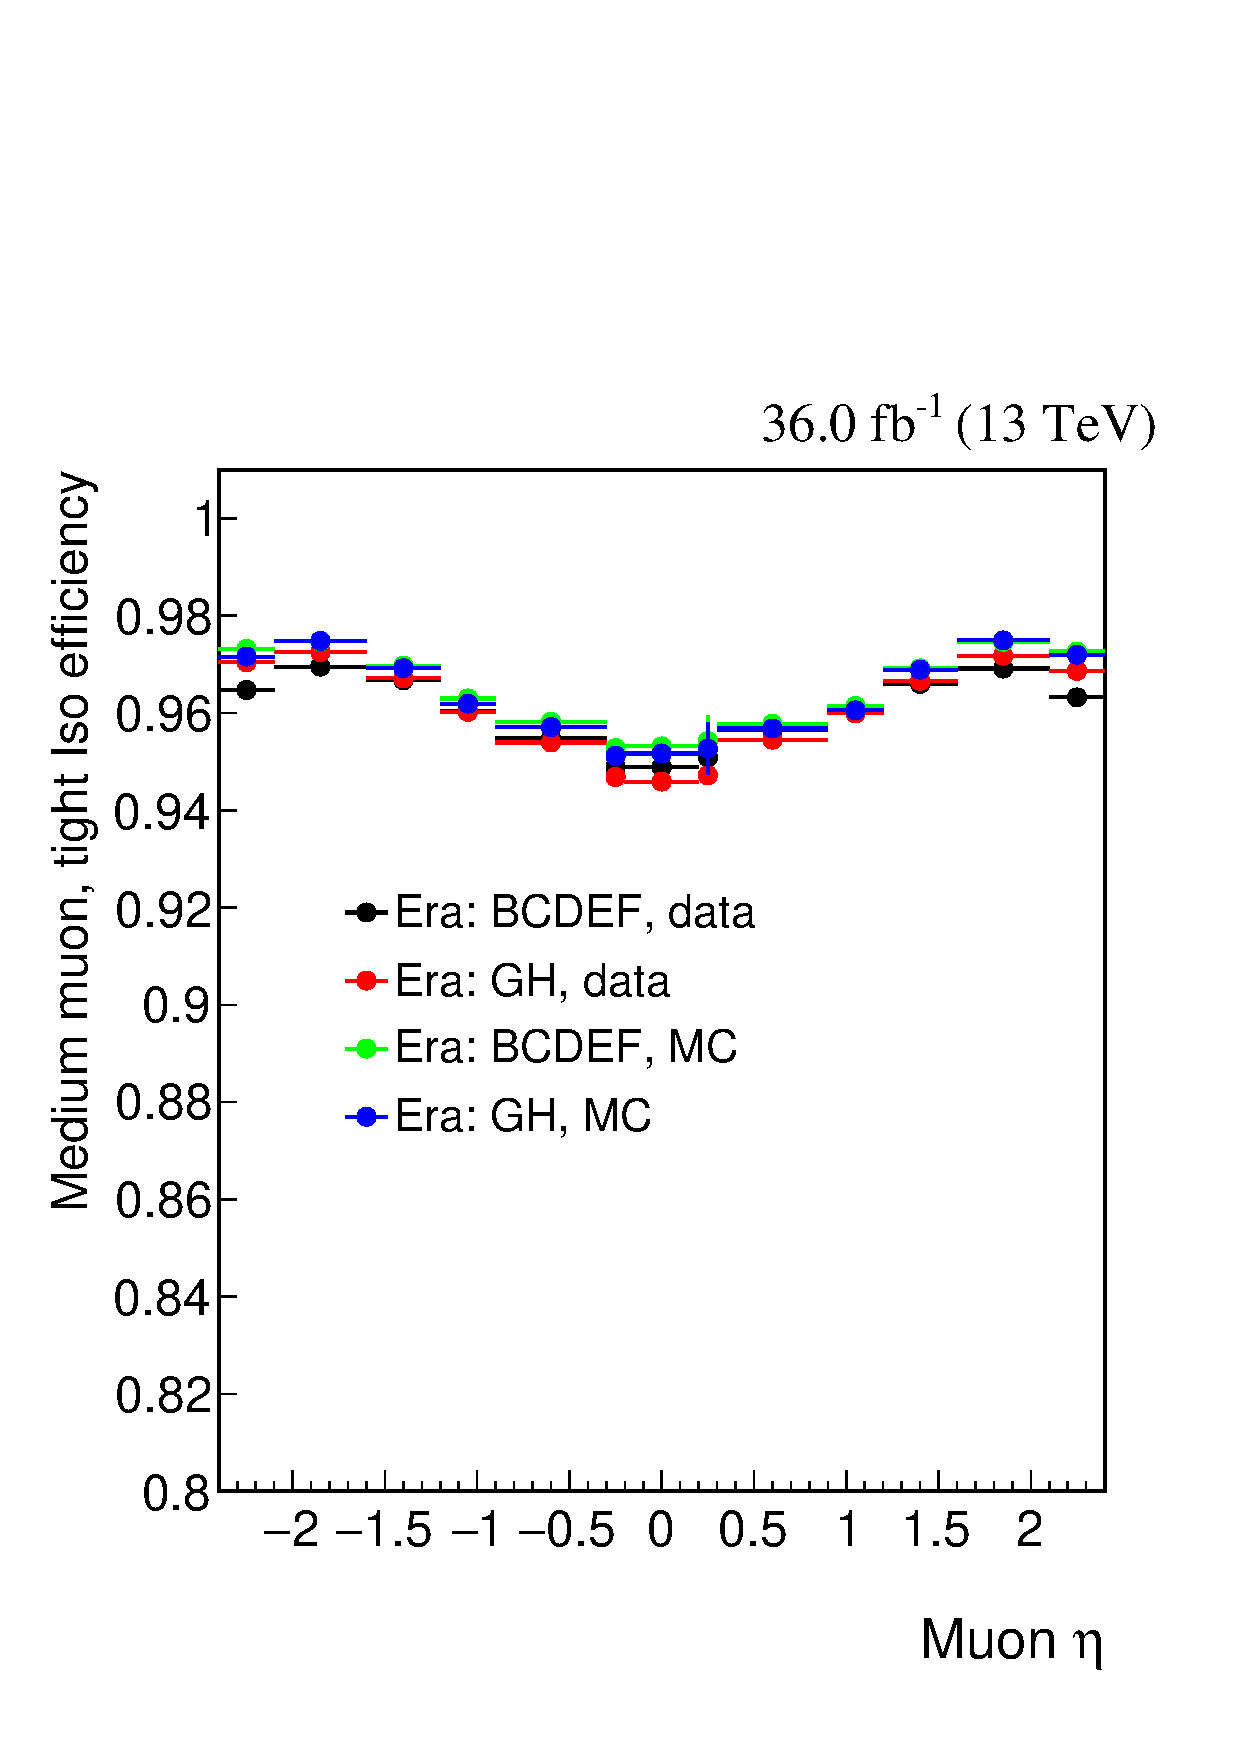
\includegraphics[width=0.45\linewidth]{Image/Muon/muSF_png/muonIsoEffEta.pdf}}
    \caption{ The distribution of efficiencies for medium muon ID and tight relative
    isolation (with medium ID) as a function of \pt and $\eta$ of muon from simulation 
    and data from different eras of 2016 data taking.}
    \label{fig:muonIsoIDEff}
\end{figure}

\subsection{Rochester correction}
Due to misalignment of the magnetic field and azimuth dependent in-efficiency of 
the muon detector, the efficiency of the muon needs to be corrected. The efficiency
depends on the charge, \pt, $\eta$ and $\phi$ of muon. These corrections referred as 
Rochester corrections are applied on data as well as simulated samples. The muon $\pt$ is
corrected using Rochester correction tools at 13 \TeV~\cite{Bodek:2012id}.
The Rochester scale factors depend on the $\pt$, $\eta$, $\phi$ and charge of the 
muon. Selection criteria (Table~\ref{tab:muonSel}) on muon are applied after 
Rochester correction.

\subsection{Isolation}
A muon track in the proton-proton collision is not necessarily isolated \ie, it can be 
surrounded by other particles. On the other hand, muons from the \PW decay are 
expected to be isolated. To achieve this, we apply a criterion on the relative
isolation, defined as the $\pt$ sum of all particles excluding the muon within a 
cone of radius 0.4 around the muon direction divided by the muon $\pt$ i.e.
$I_{\text{rel}}^\mu=\sum_{i\neq\mu}\pt^i/\pt^\mu$. We use a more specific definition given by  
\begin{equation}
\label{eq:mu_iso}
I_{\text{rel}}^\mu=\frac{\sum\pt^{\text{ch}}+{\text{max}}[(\sum E_T^\gamma+\sum E_T^{\text{neut}}-0.5\times\sum\pt^{\text{chPU}}),0]}{\pt^\mu},
\end{equation}
where $\pt^{\text{ch}}$ is the transverse momentum of charged hadrons; $E_T^\gamma$ and
$E_{T}^{\text{neut}}$ are the transverse energy of photons and neutral hadrons; and
$\pt^{\text{chPU}}$ is the transverse momentum of charged hadrons associated with the
pileup vertices. The factor $0.5$ takes into account the neutral tracks from the
leading vertex and charged tracks from the pileup vertices~\cite{Sirunyan:2018fpa}.
A tight muon isolation cut of $I_{\text{rel}}^\mu < 0.15$ is applied. The efficiency
as a function of \pt and $\eta$ of tight muon isolation with medium ID is shown in
Figure~\ref{fig:muonIsoIDEff} \cite{muSF}.

%--------------------------------------
% Electron Reconstruction
%--------------------------------------
\section{Electron }
\label{s:eleReco}
\subsection{Reconstruction}
Electrons are also reconstructed using the PF algorithm~\cite{CMS-PAS-PFT-09-001, CMS-PAS-PFT-10-001} 
based on the tracks in the tracker and energy deposits in the electromagnetic calorimeter
~\cite{Khachatryan:2015hwa}. Being a charged particle electrons radiate as they travel inside the huge
magnetic field of the CMS. Thus the energy deposited by an electron in the ECAL is
spread in $\eta$ and $\phi$ direction across several crystals. The energy deposited
in various crystals are clustered using \dq{hybrid} algorithm in the barrel and \dq{multi-5x5}
in endcap part of the ECAL. For given hits in the innermost layer of the tracker, the 
KF technique is used to find hits in the next layer of the tracker. The hits collected from all layers 
of the tracker is mapped to the energy deposit in the ECAL to form 
an electron candidate. To take care of the effect of bremsstrahlung, the Gaussian sum 
filter (GSF) method is used to fit the tracks. The electron charge is estimated from the 
curvature of the electron track and by matching associated KF track with GSF tracks. The vector joining (supercluster, beamspot) and (supercluster, first hit of the GSF track) in $\phi$ is also used for
electron charge estimation. The measurements from tracker and ECAL are combined to estimate
the electron momentum~\cite{Khachatryan:2015hwa}.

\subsection{Identification and selection}
To select a prompt electron, medium cut-based ID as listed in Table~\ref{tab:eleSel} is
used. Events having an electron with $\pt > 30$\,\GeV and $|\eta| <$ 2.5 are excluded. 
\begin{table}
  \caption{Selection and veto cuts applied on electron found in barrel and endcap regions.}
 \label{tab:eleSel}
 \centering
\begin{adjustbox}{max width=\textwidth}
 \begin{tabular}{ccccc}\hline\hline
 Variable & \multicolumn{2}{c}{Selection} & \multicolumn{2}{c}{Veto}\\
  & $|\eta_{\rm {sc}}|\leq 1.479$ & $|\eta_{\rm {sc}}|>1.479$ & $|\eta_{\rm {sc}}|\leq 1.479$ & $|\eta_{\rm {sc}}|>1.479$\\\hline\hline
 \pt (\GeV) & $> 30$ & $> 30$ & $> 15$ & $> 15$\\
 $|\eta|$ & $< 2.5$ & $< 2.5$ & $ -$ & $- $\\
 full $5\times 5$ $\sigma_{i\eta i\eta}$    & $< 0.00998$   & $< 0.0298$    & $< 0.0115 $   & $<0.037$\\
 $|\Delta\eta({\rm {sc}},{\rm {track}})|$       & $< 0.00311$   & $< 0.00609$   & $< 0.00749$   & $<0.00895$\\
 $|\Delta\phi({\rm {sc}},{\rm {track}})|$       & $< 0.103$     & $< 0.045$     & $< 0.228$     & $< 0.213$\\
 $E_{{\rm {had}}}/E_{{\rm {em}}}$               & $< 0.253$     & $< 0.0878$    & $< 0.356$     & $<0.211$\\
 $I_{\rm {rel}}^e$                            & $< 0.0821$    & $< 0.0695$    & $< 0.175$    & $<0.159$\\
 $|\frac{1}{E}-\frac{1}{p}|$ (\GeV)$^{-1}$   & $< 0.134$     & $< 0.13$      & $< 0.299$ &$<0.15$\\
 Missing inner hits                         & $\le 1$       & $\le 1$       & $\le 2$       & $\le 3$\\
 Conversion veto                            & Yes           & Yes           & Yes           & Yes\\
 $|d_{xy}({\rm {vertex}})|$ (\unit{cm})              & $< 0.05$      & $< 0.10$       &$<0.05$      & $<0.05$\\
 $|d_z({\rm {vertex}})|$ (\unit{cm})                 & $< 0.10$      & $< 0.20$       & $<0.1$      &$<0.1$\\\hline
 \end{tabular}
\end{adjustbox}
 \end{table}

A brief description of the variables listed in Table~\ref{tab:eleSel} is given below:
\begin{itemize}[leftmargin=*]
    \item full $5\times 5$ $\sigma_{i\eta i\eta}$ is defined as~\cite{Khachatryan:2015hwa} 
    \begin{equation}
    \sigma_{i\eta i\eta}=\sqrt{\sum(0.0175\times\eta_i+\eta^{\rm {seed}}_{\rm {cryst}}-\bar{\eta}_{5\times 5})^2\times w_i]/\sum w_i}, \quad w_i = 4.2 + \log(E_i/E_{5\times 5}),
    \label{eq:sIeIe}
    \end{equation}
    the summation is carried over the $5\times 5$ matrix around the highest $E_T$ crystal of the supercluster (\rm{sc}).
    \item $|\Delta\eta({\rm {sc}},{\rm {track}})|$: Difference in $\eta$ of the supercluster and the electron track.
    \item $|\Delta\phi({\rm {sc}},{\rm {track}})|$: Difference in $\phi$ of the supercluster and the electron track.
    \item $E_{\rm {had}}/E_{\rm {em}}$: Ratio of the electron energy deposited in the HCAL and ECAL.
    \item $|\frac{1}{E}-\frac{1}{p}|$: $E$ is the energy of the supercluster and $p$ is the track momentum at
    the point of closest approach from the PV.
    \item Missing inner hits: Number of missing hits in the strip tracker.
    \item $|d_{xy}({\rm {vertex}})|$: Distance of closest approach of the electron track from the PV in the $xy$ plane.
    \item $|d_{z}({\rm {vertex}})|$: Difference in the $z$-coordinate of the PV and the electron track.
\end{itemize}
The relative isolation $I_{\rm {rel}}^e$ and conversion veto of Table~\ref{tab:eleSel}
are discussed in Sections~\ref{s:ele_iso} and \ref{s:ele_conv_rej}. The efficiency of medium and 
veto electron ID as a function of \pt and $\eta$ is shown in Figure~\ref{fig:eleIDEff} \cite{eleSF}.
\begin{center}
\begin{figure}
   \subfigure[Efficiency for medium ID]
   {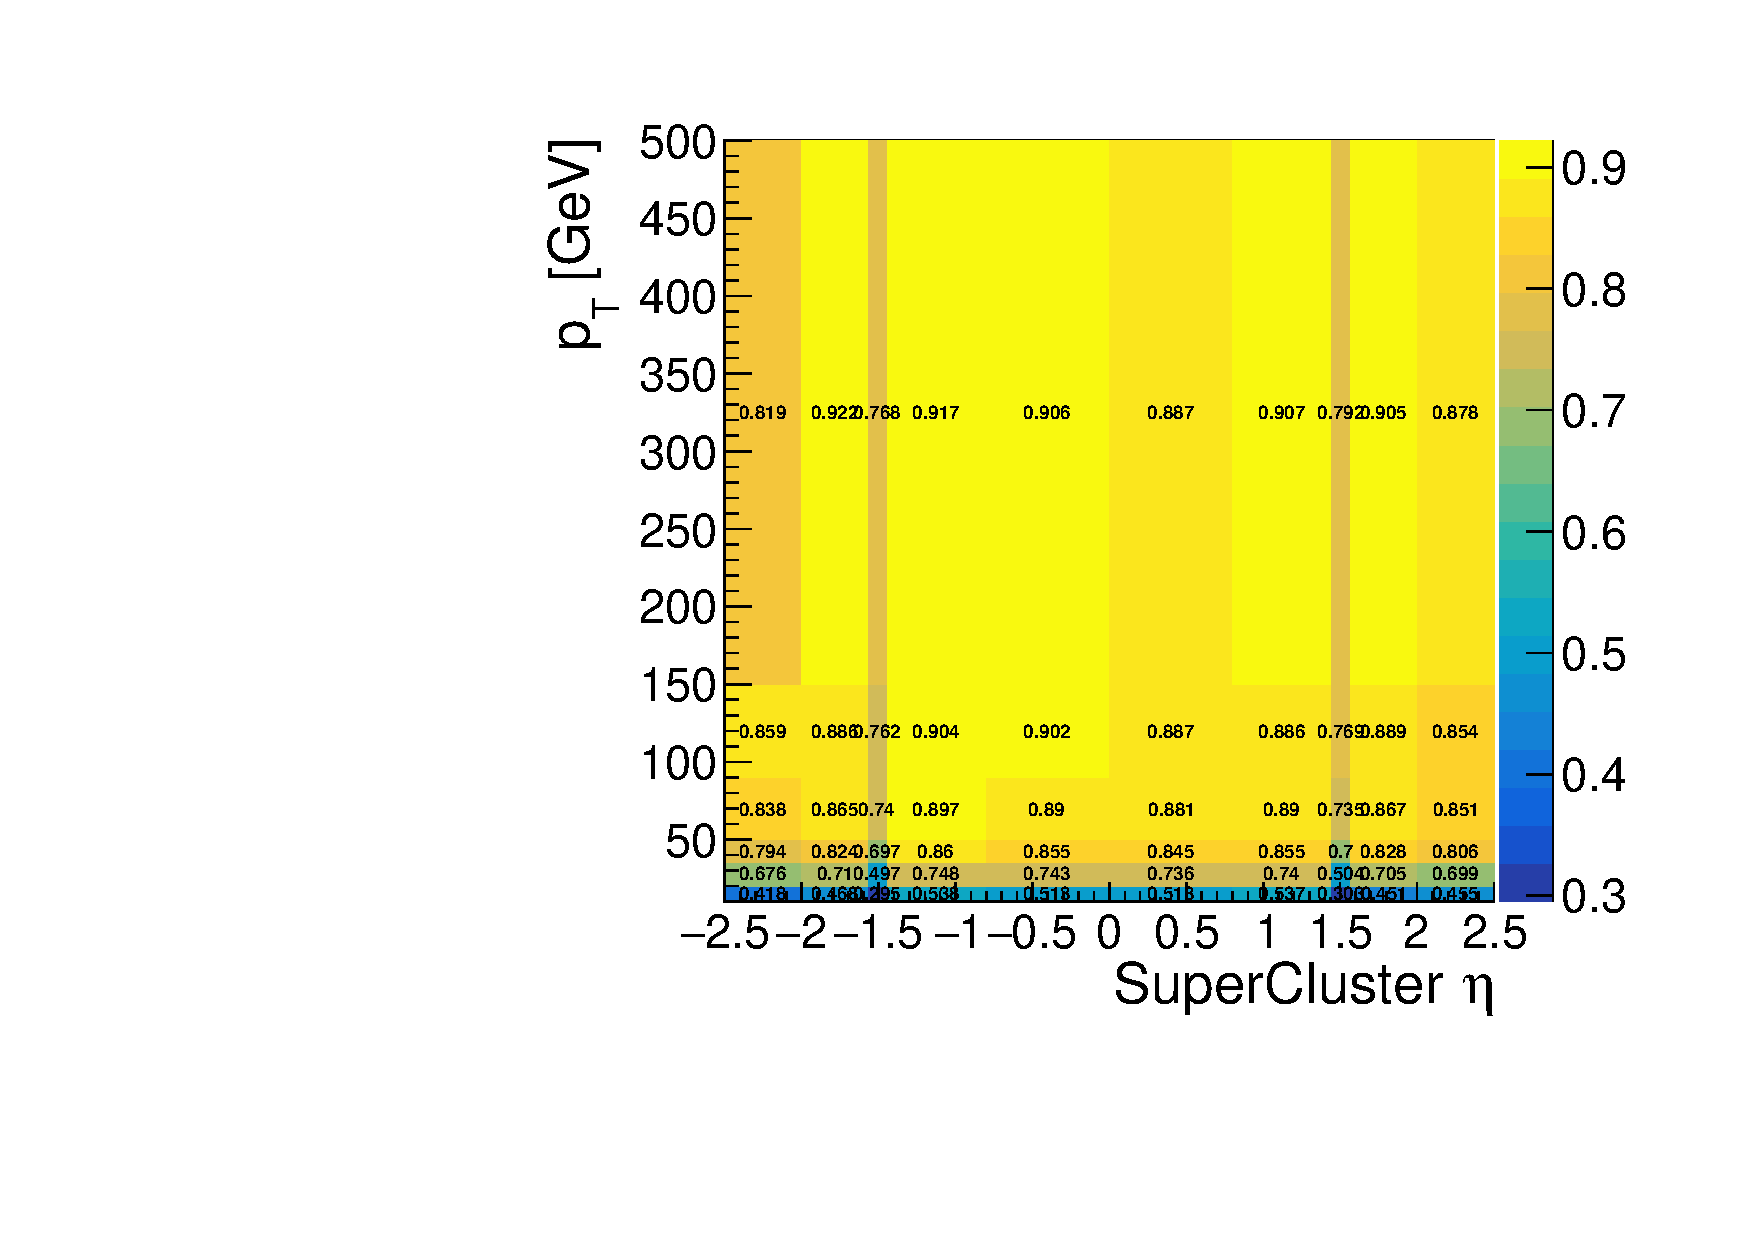
\includegraphics[width=0.49\linewidth]{Image/Electron/eleSF_png/eleMediumIDEff_mc2D.pdf}}
   \subfigure[Efficiency for veto ID]
   {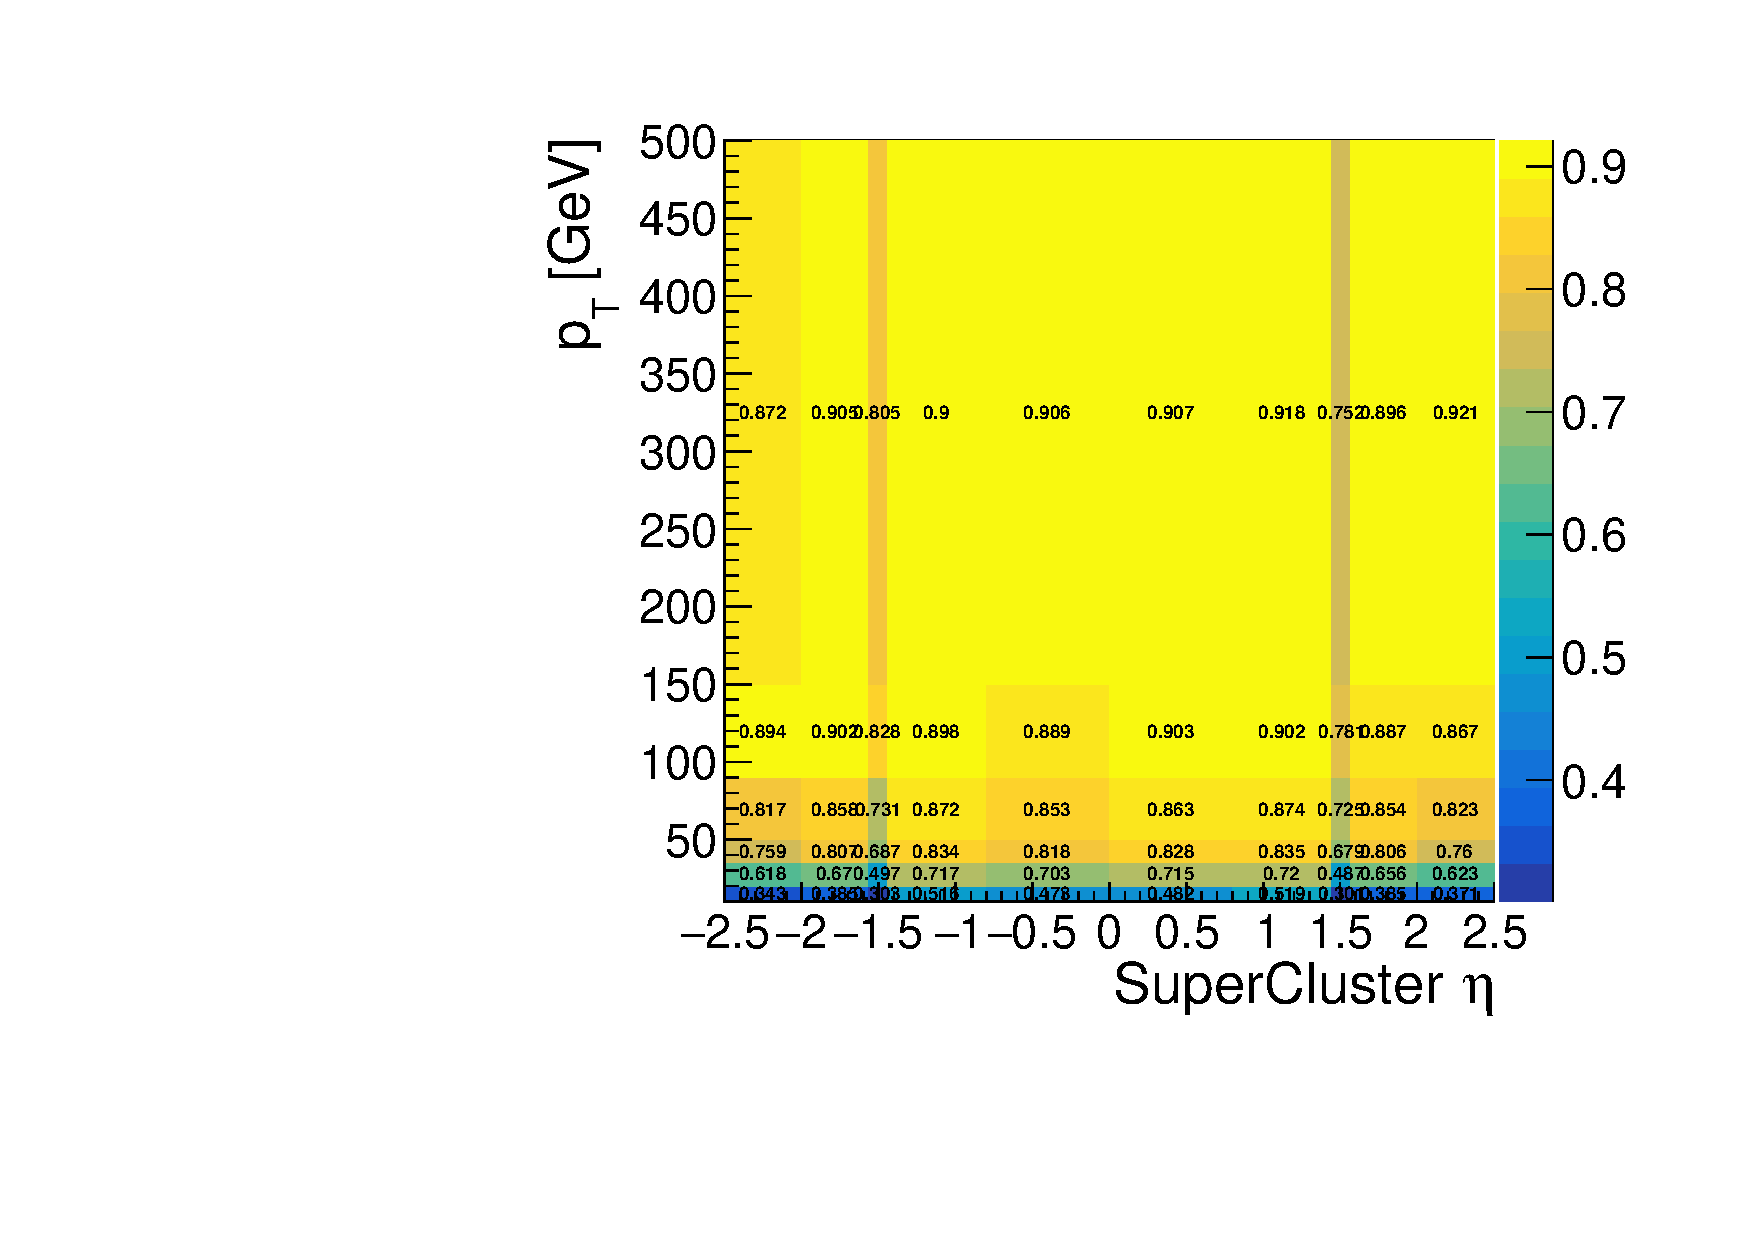
\includegraphics[width=0.49\linewidth]{Image/Electron/eleSF_png/eleMediumIDEff_data2D.pdf}}
\caption{ The distribution of efficiency for medium and veto electron ID.} 
\label{fig:eleIDEff}
\end{figure}
\end{center}

\subsection{Isolation}
\label{s:ele_iso}
The relative isolation of an electron is given by:
\begin{equation}
\label{eq:ele_iso}
I_{\rm {rel}}^e= \frac{\sum\pt^{ch}+{\rm {max}}[(\sum E_T^\gamma+\sum E_T^{\rm {neut}}-\rho\times A_{\rm {eff}}),0]}{\pt^e},
\end{equation}
where $\rho$ is as defined in Equation (\ref{eq:rho}) and $A_{\rm {eff}}$ is the 
effective area. These two quantities are used to correct electron isolation from 
pileup. The effective area for different $\eta_{\rm {sc}}$ are shown in 
Table~\ref{tab:EA}. The tight isolation cut of $I_{\rm {rel}}^e < 0.0821 ~(0.0695)$ 
is applied on electrons from the barrel (endcap) region.
\begin{table}
 \caption{Effective area for different $\eta_{\rm {sc}}$ range.}
 \begin{center}
 \begin{tabular}{cc}\hline\hline
     Super-cluster eta $(\eta_{\rm {sc}}$) & $A_{\rm {eff}}$ \\ \hline\hline
     $0.0 \leq \eta_{\rm {sc}} < 1.0 $ & $0.1703$ \\
     $1.0 \leq \eta_{\rm {sc}} < 1.5 $ & $0.1715$ \\
     $1.5 \leq \eta_{\rm {sc}} < 2.0 $ & $0.1213$ \\
     $2.0 \leq \eta_{\rm {sc}} < 2.2 $ & $0.1230$ \\
     $2.2 \leq \eta_{\rm {sc}} < 2.3 $ & $0.1635$ \\
     $2.3 \leq \eta_{\rm {sc}} < 2.4 $ & $0.1703$ \\
     $2.4 \leq \eta_{\rm {sc}} $ & $0.2393$ \\\hline
 \end{tabular}
 \end{center}
 \label{tab:EA}
 \end{table}

\subsection{Conversion rejection}
\label{s:ele_conv_rej}
Some of the reconstructed electrons are end products of photon conversion inside the tracker.
While selecting prompt electrons these secondary electrons need to be rejected.
As the secondary electrons don't have hits in the innermost layer of the tracker~\cite{Khachatryan:2015hwa},
one can use this feature to reject them.
By fitting the electron tracks, these secondary electrons are also rejected ~\cite{Khachatryan:2015hwa}.

%--------------------------------------
% Jet Reconstruction
%--------------------------------------
\section{Jet}
\label{s:jet_reco}
\subsection{Reconstruction}
Due to color confinement~\cite{Polyakov:1976fu}, the quarks and gluons produced in proton-proton 
collisions cannot exist in the free states. Instead, they hadronise into a cluster of colorless particles 
such as hadrons, leptons, and photons. We form a jet out of these particles, emanating in a cone 
around the initial direction of quarks and gluons. In CMS, the PF algorithm is used to reconstruct all 
possible particles that can be inside a jet. Subsequently, the clustering of, or the reconstruction 
of jets from, these particles are done with the anti-\kt algorithm~\cite{Cacciari:2008gp}. 

\subsection{Identification and selection}
\label{ss:jet_id}
The selection criteria applied on jets are listed in Table~\ref{tab:jetSel}.
The identification of \PQb and \PQc jet are discussed in Sections~\ref{s:bTag} and \ref{s:cTag}. 
\begin{table}
  \caption{Selection criteria applied on jets.}
 \begin{center}
 \begin{tabular}{cc}\hline\hline
 Variable & selection \\ \hline\hline
 $\pt$ (\GeV) & $> 25$ \\
 $|\eta|$ & $< 2.4$  \\
 Neutral hadron energy fraction & $<0.99$ \\
 Neutral electromagnetic energy fraction & $<0.99$\\
 Number of constituent & $ > 1$\\ 
 Charged hadron energy fraction & $ >0$ \\
 Charged hadron multiplicity & $> 0$ \\
 Charged hadron electromagnetic energy fraction & $ < 0.99$\\\hline
 \end{tabular}
 \end{center}
 \label{tab:jetSel}
 \end{table}
The charged hadron subtraction technique ~\cite{CMS-PAS-JME-14-001} is used to 
take care of the pileup effects. It ignores the charged particles coming from 
the pileup vertices. The jet energy in data and simulated samples are corrected 
to account for the non-linear response of the ECAL and HCAL. A set of corrections
are applied in a factored manner, that is, the output of previous serves as the 
input to the next step. The raw \pt of a jet is corrected at every step and the
corrected \pt is used in the subsequent analysis. These set of corrections are 
known as \verb|L1FastJet| (pileup correction through offset energy density)
\verb|L2RelativeL3Absolute| (detector response corrections), and 
\verb|L2L3Residual| (residual corrections on data). The first two are applied 
on simulated samples whereas all the three are applied on data. 
Furthermore, the jet \pt in the simulation are smeared to have same resolution as 
that of data using the jet energy resolution (JER) scale factors. Before applying 
the selection cuts listed in Table~\ref{tab:jetSel}, the jet \pt is corrected as 
discussed in Section~\ref{s:JEC}. 

\subsection{Cleaning}
The prompt leptons (electrons and muons) are required to be outside the jet cone.
This procedure is called jet cleaning, where we require the angular separation between the
jet and lepton, $\Delta \rm R > 0.5$.

%--------------------------------------
% \MET Reconstruction
%--------------------------------------
\section{Missing transverse energy}
\label{s:secMET}
The missing transverse energy (\MET) is the negative vector sum of the momenta of all objects
reconstructed with the PF algorithm.
Being a weakly interacting particle, neutrinos are not directly detected through the CMS
detector and thus contribute to \MET.
Note that this is not true only for the SM; there are some beyond-the-SM particles e.g.,
neutralinos in supersymmetry that could also contribute to \MET.
Nevertheless, as there is a neutrino in our signal events (see Figure~\ref{fig:feyn_diag_sig})
we expect large \MET due to its escape from the detector.
The \MET in simulation and data can have different resolutions. Therefore, \MET from simulated events 
are smeared using the \verb|Type-1| correction in which jet energy correction is propagated to the 
\MET. The events having \MET $>$ 20 \GeV are selected as described in Section~\ref{s:secEvtSel}.
